\section{ZigBee}

ZigBee is a widely used wireless communication technology designed for low-power, low-data-rate applications. 

\paragraph*{History}
In the mid-1990s, IoT solutions were highly fragmented, with numerous proprietary protocols leading to major compatibility and interoperability challenges. 
This also drove up costs, making large-scale adoption difficult.
To address this, IEEE launched Working Group 4 in 2001 to develop a standardized reference technology. 
This effort resulted in the IEEE 802.15.4 standard, which was officially published in March 2003.

\begin{figure}[H]
    \centering
    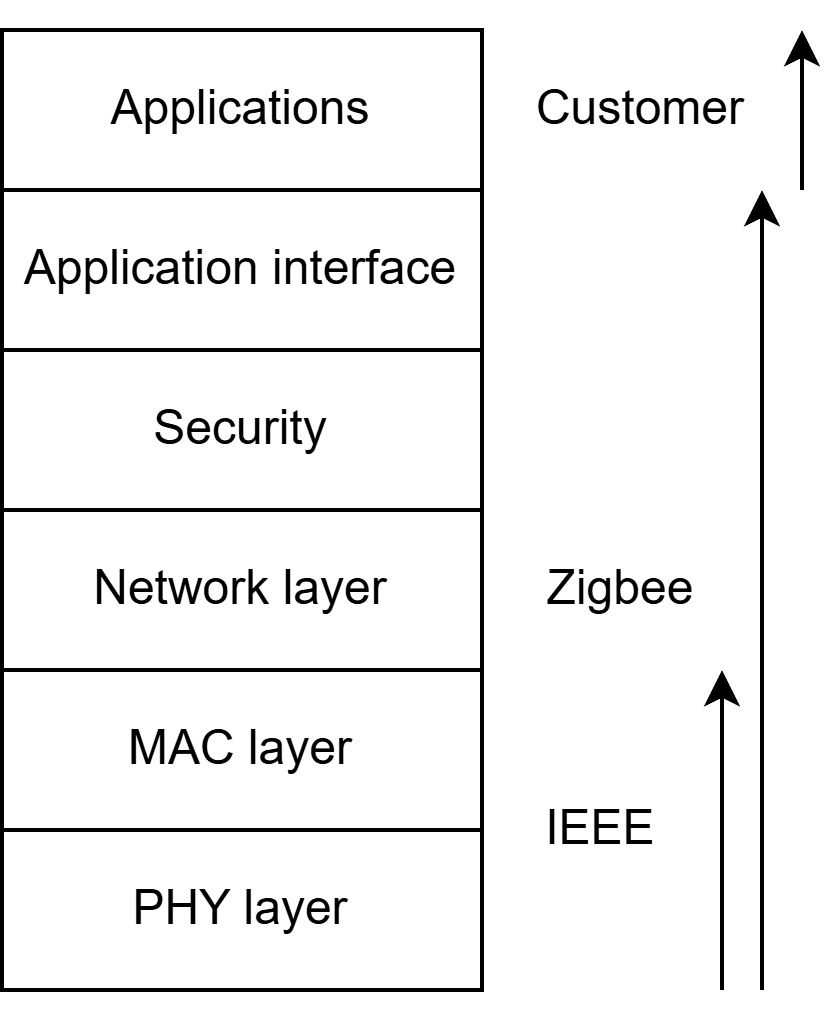
\includegraphics[width=0.3\linewidth]{images/iot14.png}
    \caption{ZigBee communication stack}
\end{figure}

\paragraph*{Taxonomy}
ZigBee networks consist of different types of devices, each playing a specific role:
\begin{itemize}
    \item \textit{Full function device}: can send beacons to manage network communication, communicate with other FFDs, route network frames, and act as a PAN coordinator. 
        Typically powered by an external power supply.
    \item \textit{Reduced function device}: cannot route frames or communicate with other RFDs.
        Communicates only with an FFD.
        Designed for low-power, battery-operated applications.
    \item \textit{PAN coordinator}: handles device association and de-association.
\end{itemize}
\noindent ZigBee networks support three different topologies, each suited for specific use cases:
\begin{itemize}
    \item \textit{Star topology}: all devices connect to a central coordinator.
        Simple, but limited in scalability.
        Common in home automation and industrial monitoring.
    \item \textit{Mesh topology}: devices communicate with multiple neighboring nodes.
        Highly reliable and scalable, as data can take multiple paths.
        Used in large-scale IoT deployments.
    \item \textit{Cluster-tree topology}: an hybrid between star and mesh.
        Devices are organized in clusters, with a coordinator managing each cluster.
        Efficient for applications requiring structured hierarchies, such as industrial automation.
\end{itemize}

\subsection{Physical layer}
The physical layer (PHY) of ZigBee, based on IEEE 802.15.4, is responsible for managing radio communication and ensuring reliable data transmission. 
Its main functions include: radio transceiver control, energy detection, link quality indicator, clear channel assessment, channel frequency selection, and data transmission and reception.
ZigBee operates across multiple frequency bands, offering flexibility based on regional regulations and application requirements: 868 MHz, 915 MHz, and 2.4 GHz. 

\subsubsection{Medium Access Control layer}
The MAC sub-layer provides key functionalities such as: beacon management, channel access management, guaranteed time slot management, frame validation, acknowledged frame delivery, association and disassociation, and sSecurity hooks.
ZigBee defines two operation modes to balance power efficiency and communication reliability:
\begin{enumerate}
    \item \textit{Beacon-enabled mode}: the PAN Coordinator periodically transmits beacons to synchronize devices.
        Commonly used in star topologies.
        Uses a combination of slotted CSMA-CA and scheduled transmissions to manage channel access.
    \item \textit{Non beacon-enabled mode}: devices communicate using un-slotted CSMA-CA, meaning no predefined transmission schedule.
        Provides uncoordinated access, reducing overhead but increasing the risk of collisions.
\end{enumerate}

\paragraph*{Channel access mechanism}
Since multiple devices share the same frequency, ZigBee uses a mix of scheduled and random access to prevent interference:
\begin{itemize}
    \item \textit{Scheduled Access}: managed by the PAN Coordinator (only in beacon-enabled mode).
    \item \textit{Random Access}: used for communication between RFDs or between RFD/FFD and the PAN Coordinator.
        Allowed in both operation modes.
\end{itemize}

\subsubsection{CSMA/CA}
ZigBee devices rely on CSMA/CA to reduce transmission conflicts. 
Each device tracks key variables to manage communication: 
\begin{itemize}
    \item The number of back-offs, which counts transmission delays.
    \item The contention window, controlling how long the channel must remain clear before transmission.
    \item The backoff exponent, determining the wait time before attempting access.
\end{itemize}
\noindent The CSMA/CA process begins with the transmitting node waiting for a random backoff period. 
If the channel remains clear for the required CW duration, the device proceeds with transmission and awaits an acknowledgment. 
However, if the channel is busy, the node increases both BE and NB, repeating the process until either a successful transmission occurs or the retry limit is reached, at which point the packet is discarded.
All transmissions, including ACKs, must complete within the Contention Access Period. 
While slotted CSMA/CA requires synchronization, un-slotted CSMA/CA operates without it. 
Certain packets bypass CSMA entirely and transmit immediately. 
If a collision occurs the device restarts the procedure.

\subsubsection{Network formation}
To join a network, ZigBee devices scan for available PANs: 
\begin{itemize}
    \item Active scanning, used by full-function devices, involves sending a beacon request, prompting nearby PAN coordinators to respond with beacons. 
        After scanning, the device selects a PAN ID and joins. 
    \item Passive scanning, available to both FFDs and reduced-function devices, operates similarly but without actively requesting beacons.
        Instead, the device listens for beacon transmissions from coordinators.
\end{itemize}

\subsubsection{Extensions}
Enhancements to the IEEE 802.15.4 standard have expanded ZigBee's capabilities for specialized applications.
IEEE 802.15.4e introduces slotted channel access for improved efficiency. 
IEEE 802.15.4g targets smart utility applications while IEEE 802.15.4k optimizes communication for critical infrastructure monitoring, including power grids and industrial control systems.

\subsection{Network layer}
The network layer provides is used to: configure anew device, start a network, join and leave a network, address, neighbor discovery, route discovery, reception control, and routing.
In ZigBee, there are three types of devices:
\begin{itemize}
    \item \textit{ZB coordinator} (FFD): the central coordinator that initiates and manages the network.
    \item \textit{ZB router} (FFD): routers that relay messages and allow other devices to join the network.
    \item \textit{ZB end-device} (RFD or FFD): end devices.
\end{itemize}
\noindent ZigBee routing integrates two primary protocols: Ad-hoc On-demand Distance Vector (AODV) and cluster tree algorithm. 

\subsubsection{Cluster tree algorithm}
The cluster tree algorithm defines how a ZigBee network organizes itself into a tree structure for efficient data routing.
The most important operations are: 
\begin{itemize}
    \item \textit{Tree initialization by FFD}: a ZigBee FFD begins the tree formation by scanning available channels and selecting one with minimal interference. 
        It sets its PAN identifier and assigns itself the network address 0, indicating its role as the coordinator.
        The ZigBee coordinator fixes the maximum number of routers ($R_m$), end-devices ($D_m$) that each router may have as children and the maximum depth of the tree ($L_m$).
    \item \textit{Association of devices}: other devices can then join the network by associating with the coordinator through standard association procedures. 
        These devices may be routers or end-devices.
    \item \textit{Address assignment}: during the association process, devices are assigned 16-bit short addresses. 
        The parent device assigns address ranges to its child devices. 
        Each router receives a consecutive block of addresses based on its depth in the tree, while the first address in this block is used as the node's address, and the remaining addresses are available for its child devices.
        The size of the address range $A(d)$ assigned to a router node at depth is calculated using the following formula:
        \[A(d)=\begin{cases} 1+D_m+R_m\qquad\qquad\qquad\text{if }d=L_m-1 \\ 1+D_m+R_mA(d+1)\:\qquad\text{if }0 \leq d <L_m-1 \end{cases}\]
\end{itemize}
Routing within a ZigBee network follows the tree structure formed by the coordinator and its child devices. 
Messages are routed through the tree in the following manner:
\begin{itemize}
    \item If the destination address belongs to one of the child end-devices, the message is routed directly to the destination.
    \item If the destination address corresponds to a child router, the message is sent to that router for further forwarding.
    \item If the destination address is not found among the children, the message is forwarded to the parent node for further routing.
\end{itemize}

\subsubsection{Ad-hoc On-demand Distance Vector}
AODV is a reactive routing protocol used when a device needs to send data to an unknown destination. 
Here's how AODV works:
\begin{enumerate}
    \item \textit{Route request} (RREQ): when a device wants to communicate with a destination, it broadcasts a RREQ message.
    \item \textit{Flooding}: the RREQ message is flooded across the network, and each node that relays the request stores the address of the node that forwarded it, setting up a reverse path to the source.
    \item \textit{Route reply} (RREP): when the destination node receives the RREQ, it sends a RREP message back to the source, traveling along the reverse path set up during the flooding process.
\end{enumerate}
\noindent Routing tables are updated as nodes process these RREQ and RREP messages. 
A node's routing table contains the destination address, the nex-hop address and the entry status (active or not).
Additionally, a Routing Discovery Table (RDT) keeps track of RREQ messages.

\paragraph*{Routing cost}
The cost of a path $P$ is the sum of the individual costs of the links that make up the path: 
\[C\{P\}=\sum_{i=1}^{L-1}C\left\{\left[D_i,D_{i+1}\right]\right\}\]
\noindent The cost for each link $l$ follows a standard cost function: 
\[C(l)=\begin{cases}7\\\min\left(7,\text{round}\left(\dfrac{1}{p_l^4}\right)\right)\end{cases}\]

\subsection{Application profiles}
ZigBee also provides predefined application profiles that ensure interoperability across different devices and manufacturers. 
These profiles define a common language for data exchange with a set of processing actions for devices.
This allows device interoperability across manufacturers and simplicity and reliability for end users.
Each profile is made up of:
\begin{itemize}
    \item A set of devices needed for the application.
    \item A set of clusters that implement the required functionality.
    \item A set of attributes representing device state.
    \item A set of commands enabling communication between devices.
\end{itemize}